\chapter{Computational Models for Encoding Natural Images}


\section{Introduction}
Motivation for sparse coding, taking generative approach, uncertainty, etc.
Sparse coding is a generative model for explaining natural signals. The model has been implemented for coding several different signal modalities \parencite{placeholder} and related to multiple brain regions \parencite{placeholder}. However, here we will focus on coding of images in the context of computation being performed by layer 4 cells in V1.

We will begin this chapter with a probabilistic derivation for the sparse coding model. Importantly, this will make clear the various assumptions built into the model, which will be relevant for our interpretations of results in later chapters. The first section will get us to an energy function that a sparse coding algorithm would seek to minimize. The second section recapitulates the sparse coding model from an optimization perspective and outlines standard methods for inference and dictionary learning. Next, we will derive the Locally Competitive Algorithm, which is a neural network model designed to perform sparse inference. This network is the subject of the rest of the thesis. Finally, we will compare the LCA model to other popular neurally-inspired image coding models, namely Predictive Coding \parencite{rao1999predictive} and ICA \parencite{bell1997independent}.

\section{A probabilistic approach for image coding}
We aim to encode an incoming signal efficiently under the assumption that the signal is composed of a structured component and unstructured additive noise. We do this with sparse coding, which assumes a linear generative model:

\begin{equation} \label{eq:ch2_generative_model}
    s = \Phi a + \varepsilon,
\end{equation}

\noindent where $s$ is our input signal, $\Phi$ is an overcomplete (in that the number of columns in $\Phi$ is greater than the number of rows) dictionary of functions, $a$ is a row vector of activation coefficients, and $\varepsilon$ is Gaussian noise. For a given input signal, the task of finding an optimal set of coefficients is ill-posed. This is partially because the noise is unknown and therefore cannot be completely accounted for. Another reason is that the dictionary is overcomplete and thus non-orthogonal, resulting in an infinite number of possible combinations that are each equally valid representations. Following the work of \parencite{olshausen1996learning} and \parencite{karklin1999porbabilistic}, we will derive a probabilistic generative model for computing image codes with an optimality constraint in the form of sparsity. Additionally, we can follow a similar derivation to learn a set of dictionary elements that maximize coding efficiency.

Our model assumes a prior probability over the images, $P(s)$, and the activity coefficients, $P(a)$. We also assume that the coefficient prior does not depend on the dictionary itself, that is $P(a|\Phi) = P(a)$. Although in practice the coefficients and dictionary will be jointly optimized, we can adhere to this assumption by fixing one variable while optimizing the other in an expectation-maximization like procedure. We specify the likelihood of an image under the model for a given state of coefficients as $P(s|a,\Phi)$. Conversely, given evidence in the form of an image sample, we can define the posterior as the conditional probability distribution of our coefficients given the image and model: $P(a|s,\Phi)$. Our goal is to maximize this posterior distribution, which gives us the most probable estimate of the coefficients. As is done in \parencite{karklin1999porbabilistic}, we can relate the likelihood and posterior using Bayes' rule:

\begin{equation}\label{eq:ch2_bayes}
    P(a|s,\Phi) \propto P(s|a,\Phi) P(a)
\end{equation}

The probability of the image under the model, $P(s|\Phi)$ is obtained by marginalizing over the internal states:

\begin{equation}\label{eq:ch2_image_probability}
    P(s|\Phi) = \int\partial a P(s|a,\Phi) P(a)
\end{equation}

In the sparse coding model we assume that the noise distribution is Gaussian. We justify this by assuming that the generative model can account for everything except for random, uncorrelated (i.e. independent) causes that combine in the limit to follow a Gaussian distribution. Under this assumption, we can specify our image likelihood:

\begin{equation}\label{eq:ch2_image_likelihood}
    P(s|a,\Phi) \propto e^{-\frac{1}{2\sigma_{i}^{2}}|s-\phi a|^{2}},
\end{equation}
\noindent where $\sigma$ is the standard deviation of the additive noise. Our goal is to encode the images as efficiently as possible, which we can define in terms of the entropy of the data: $\mathcal{L} \geq H(p) = -\sum p(x) log{p(x)}$, where $\mathcal{L}$ is the code-word length. If we assume that the mean of the image distribution exists at $\Phi a$, then the maximum entropy distribution (with infinite variance) is Laplacian, which implies a factorial distribution over our coefficients:

\begin{equation}\label{eq:ch2_coefficient_prior}
    P(a) \propto \prod_{i}\frac{1}{\lambda} e^{\frac{-|a_{i}|}{\lambda}},
\end{equation}

\noindent where $\lambda = \tfrac{1}{\sigma^{2}}$. Finally, because we are assuming the noise is Gaussian, we can impose an $L_{2}$ prior on the pixel dimension of the dictionary:

\begin{equation}\label{eq:ch2_dictionary_prior}
    P(\Phi_{i}) = \frac{1}{\sqrt{2\pi}\sigma^{2}}e^{\frac{-\sum_{j}|\Phi_{i,j}|^{2}}{\sigma^{2}}}
\end{equation}

To estimate the most likely coefficients we can maximize the posterior of the coefficients given the data and model by finding a minimum of the log-likelihood:

\begin{align}\label{eq:ch2_min_log_likelihood}
\begin{split}
    \max_{a} p(a|s,\Phi) &= \max_{a}\left[\log{P(s|a,\Phi)} + \log{P(a)}\right] \\
                         &= \min_{a}\frac{\lambda}{2}|s - \Phi a|^{2} + |a|
\end{split}
\end{align}

Ideally, we would like to maintain a distribution of probable coefficients for a given image and model. However, we will only store the most likely coefficients, which we justify by assuming that the distribution is highly peaked and therefore the maximum of the distribution is the most probable.

If we wish to find the optimal dictionary, then we will perform the same maximum-likelihood operation on equation \ref{eq:ch2_image_probability}. However, it is not tractable to integrate over the coefficients to find the marginals, so instead we use a maximum a-posteriori estimate, which approximates the area using the peak of the distribution. This is a fair estimate if the model is sure of the posterior, that is to say that $P(a|s,\Phi)$ truly follows a highly peaked distribution with heavy tails. Given this assumption, we define the log of the probability of the image under the model:

\begin{equation}\label{eq:ch2_log_image_probability}
    \log{P(s|\Phi)} = \log{\int P(s|a,\Phi)P(a)\partial a},
\end{equation}

\noindent and take the gradient with respect to our weights to give us a weight update rule:

\begin{equation}\label{eq:ch2_probability_weight_update}
    \nabla_{\Phi} \log{P(s|\Phi)} = \left< \left[s - \Phi a\right]a^{\top}\right>_{P(a|s,\Phi)}.
\end{equation}

The expectation in equation \ref{eq:ch2_probability_weight_update} tells us that we must do inference under the posterior. As we will see later, the weight and coefficient update rules can also be derived from the same energy function, which is defined as the negative log of the likelihood. The following sections give alternative derivations of the sparse coding model, which build from this probabilistic background towards a set of equations that can be optimized in a neural network framework.


\section{Sparse coding}
In practice, sparse coding on images involves the tasks of learning a dictionary from data and, given a dictionary, finding an optimal sparse code for an input signal. We define an optimal sparse code as one that gives the most faithful representation of the data using the fewest dictionary elements. The primary objective of sparse coding, as described in \parencite{olshausen1997sparse}, is to encode input data (e.g. an image of a natural scene) in a generative framework, such that the data can be reconstructed from the code. Typically, we want the encoding to be of a higher dimensionality than the input image; that is to say we want our dictionary to be overcomplete.

For an $N$-dimensional input signal (e.g. an $N$ pixel image), $s \in \mathbb{R}^{N}$, we want a dictionary of $M > N$ vectors, where each vector is of length $N$. The dictionary is a matrix $\Phi$ with dimensions $N \times M$. Each of the $M$ columns are dictionary elements, $\Phi_{i}, i \in \{1,...,M\}$, and each dictionary element has a corresponding coefficient, $a_{i}, i \in \{1,...,M\}$, that we can assemble into a vector of activations. Our goal is to minimize an energy function that requires both a faithful and efficient representation of the data, in that it reconstructs the data well with the fewest number of active elements. We can express this mathematically as

\begin{equation}\label{eq:ch2_sparse_energy}
    \argmin\limits_{a, \Phi}
        \left( E =
            \overbrace{ \tfrac{1}{2} \| s - \hat{s} \|_{2}^{2} }^\text{Preserve Information} +
        \overbrace{ \lambda \sum\limits_{i=1}^{M}C(a_{i}) }^\text{Limit Activations} \right),
\end{equation}

where $\hat{s} = \sum\limits_{i=1}^{M}\Phi_{i}a_{i}$ is the image reconstruction, $\argmin\limits_{a, \Phi}$ tells us that we want to minimize the energy with respect to both the activations and the dictionary, and $||.||_2^2$ indicates the squared $l_2$ norm. In this energy function, we use $\lambda$ as a trade-off penalty between the reconstruction quality and the sparsity constraint. Note that we have performed a change of variables from the previous section, to include the noise variance, $\sigma$ into a new $\lambda$ parameter that now modulates the $L_{1}$ cost as a Lagrange multiplier. In practice we tune it to maximize network sparsity for a minimum accepted reconstruction quality. One popular choice for the cost function, $C(.)$, is the $l_1$ cost penalty, which is the sum of the absolute value of all activations:

\begin{align}\label{eq:ch2_l1_cost}
\begin{split}
  &C(a_{i}) = |a_{i}| \\
  &\sum\limits_{i=1}^{M}C(a_{i}) = \sum\limits_{i=1}^{M}|a_{i}|
\end{split}
\end{align}

Depending on the choice of cost function, solving equation \ref{eq:ch2_sparse_energy} can be convex or non-convex. For the $l_{1}$ cost, it is non-convex. Previous work has solved this via alternating projected gradient descent \parencite{olshausen1997sparse}, basis pursuit denoising \parencite{chen2001atomic}, or matching pursuit \parencite{davis1997adaptive, rhen2007network, rebollo-neira2002Optimized}. The basis pursuit denoising variant is often accomplished using the iterative shrinkage and thresholding algorithm (ISTA) \parencite{daubechies2004iterative, beck2009fast}. Rozell et al. \citeyearpar{rozell2008sparse} proposed an alternative to ISTA using a neural network following dynamics governed by the energy gradient. The following section explains this alternative in detail.


\section{The Locally Competitive Algorithm}
The Locally Competitive Algorithm (LCA) is a method for computing a sparse code from a given input signal and dictionary. The model describes an activation coefficient, $a_{k}$, as the thresholded output of some model neuron's internal state, $u_{k}$, which is analogous to the neuron's membrane potential. This internal state follows similar dynamics to a leaky integrator neuron model. The LCA can be described as a continuous system that is implementable in hardware, or as a discrete system with an internal state that advances as a function of a time step. As the model state advances, the system relaxes to a minimum solution of the energy function described in equation \eqref{energyfunc}. Here we will derive the dynamical equation for computing the state transitions from the energy function.

We wish for our neuron activations to minimize the energy function described in equation \eqref{energyfunc}. The standard way to do this would be to perform direct gradient descent on the energy function. To illustrate the derivative, we first express the energy function in subscript notation:

\begin{equation}\label{eq:ch2_indexed_energy_func}
    E(t) = \tfrac{1}{2} \sum\limits_{i=1}^{N} \left[ S_{i} - \sum\limits_{j=1}^{M}a_{j}(t) \Phi_{i,j} \right]^{2} + \lambda \sum\limits_{j=1}^{M} C(a_{j}(t))
\end{equation}

and then we take the derivative with respect to an individual neuron's activity, $a_{k}(t)$. Since we ultimately want to do gradient \textit{descent}, we will write the negative derivative:

%\begin{equation}
\begin{align}\label{deda}
    - \frac{\partial E(t)}{\partial a_{k}(t)}
    =
        &\sum\limits_{i=1}^{N} S_{i} \Phi_{i,k} -
        \Phi_{i,k}\sum\limits_{j=1}^{M}a_{j}(t) \Phi_{i,j} -
        \lambda \sum\limits_{j=1}^{M}\frac{\partial C(a_{j}(t))}{\partial a_{k}(t)} \\
    =
        &\sum\limits_{i=1}^{N} \left[ S_{i} \Phi_{i,k} -
        \sum\limits_{j \neq k}^{M} \Phi_{i,k} \Phi_{i,j} a_{j}(t) - \Phi_{i,k}\Phi_{i,k}a_{k}(t) \right] -
        \lambda \frac{\partial C(a_{k}(t))}{\partial a_{k}(t)}
\end{align}
%\end{equation}

One constraint that we impose on our model is that we want the dictionary elements to all be unit norm in the pixel dimension, $||\phi_{i}||_2^2 = 1$. This means that the $\sum_{i=1}^{N}\Phi_{i,k}\Phi_{i,k}a_{k}(t)$ term in equation \eqref{deda} reduces to $a_k(t)$:

\begin{equation}
    -\frac{\partial E(t)}{\partial a_{k}(t)} =
    \sum\limits_{i=1}^{N} \left[ S_{i} \Phi_{i,k} -
    \sum\limits_{j \neq k}^{M} \Phi_{i,k} \Phi_{i,j} a_{j}(t) \right] - a_{k}(t) -
    \lambda \frac{\partial C(a_{k}(t))}{\partial a_{k}(t)}
\label{dedasimple}
\end{equation}

Note that $E(t)$ and $a(t)$ both vary in time. In this scenario, we can imagine a constant input signal, $S$, and a constant set of dictionary elements, $\Phi$. Given these constants, we want the system to evolve over time to produce an optimal set of activations, $a$. Equation \eqref{indexenergyfunc} gives us the energy at each time point during this inference process. Each neuron has a corresponding dictionary element, $\phi_{k}$, which is a vector that indicates the connection strength to each pixel in the input. In the literature this is also referred to as the strength of the synaptic connections between the neuron and each input pixel, or the neuron's feed-forward receptive field. In this model, we are going to find a sparse code for one patch of an image at a time, so that all $M$ neurons are connected to the same image patch, $S$. The model neuron has a driving excitatory input, which we will denote $b_{k} = S\phi_{k} = \sum_{i=1}^{N}S_{i} \Phi_{i,k}$. This is the projection of the input image onto the neuron's corresponding dictionary element. The stronger the similarity between the input, $S$, and the dictionary element, $\phi_{k}$, the stronger the driving excitatory input. Each neuron also receives inhibition from every other active neuron. The magnitude of inhibition is partially set by an $M \times M$ Gramian matrix, $G$. The matrix evaluates to the inner product of the each neuron's dictionary element with all other neurons' dictionary elements, $G = \Phi^T\Phi$, such that each element in $G$ gives the overlap in pixel space between two dictionary elements, $G_{i,j} = \sum\limits_{n=1}^{N} \Phi_{n,i}\Phi_{n,j}$. The total inhibition onto a neuron is also scaled by how active the inhibiting neuron is.

Next, we define a new function that maps the activity for a neuron and the sparsity cost function to a new scalar. This function can be thought of as the self inhibition that increases as the value of $a_{k}$ increases:

\begin{equation}\label{hopfieldtfunc}
f_{\lambda}(a_{k}(t)) = a_{k}(t) + \lambda \frac{\partial C(a_{k}(t))}{\partial a_{k}(t)}
\end{equation}

Now we can write the partial derivative of our energy function (equation \eqref{energyfunc}) in terms of our new variables:

\begin{equation}\label{dedasimple}
    - \frac{\partial E(t)}{\partial a_{k}(t)} =
    b_{k} -
    \sum\limits_{j \neq k}^{M} G_{k,j} a_{j}(t) -
    f_{\lambda}(a_{k}(t)).
\end{equation}

At this point we could update $a(t)$ using gradient descent following equation \eqref{dedasimple} to produce a sparse code from an input signal. A better solution would be to have the neuron maintain an internal state, analogous to the neuron's membrane potential. The neuron could then only produce output when its membrane potential passed over some threshold. This will have better correspondence to biology and it will give the neurons sub-threshold dynamics that will influence their activity (see section \ref{sec:section}) when compared to using equation \ref{dedasimple}. Following this logic, Rozell et al. \citeyearpar{rozell2008sparse} define an internal state variable, $u_{k}(t)$ that represents the membrane potential for neuron $k$ at time $t$. When a neuron's potential climbs above some threshold, it communicates in the form of an activation, $a_{k}(t)$. Only these excited neurons can contribute to the image code. Ultimately, the network of neurons should still descend the energy function from equation \eqref{energyfunc}, so our neuron's state dynamics must be governed by the following equation:

\begin{displaymath}
    \dot{u_{k}}(t) \propto - \frac{\partial E(t)} {\partial a_{k}(t)} \\
\end{displaymath}

\begin{equation}\label{udot}
    \dot{u_{k}}(t) = \frac{1}{\tau} \left[b_{k} - \sum_{m \neq k}^{M}G_{k,m}a_{m}(t) - f_{\lambda}(a_{k}(t)) \right],
\end{equation}

\noindent where $\tau$ is a proportionality constant that represents the time constant of the dynamics.

In order to have a complete description of the model, we need to describe a relationship between $u$ and $a$. Earlier the $f_{\lambda}(a_{k}(t))$ term was described as a self inhibition term that encourages sparsity. Another way to enforce self inhibition is to introduce a membrane leak term. If we assign the internal state, $u_{k}(t)$, to this function:

\begin{equation}\label{ufunca}
    u_k(t) = f_{\lambda}(a_{k}(t)),
\end{equation}

\noindent then we can think of our neuron as a leaky integrator. We can also invert the function to get our neuron's output activity:

\begin{displaymath}\label{athresh}
    a_{k}(t) = f_{\lambda}^{-1}(u_{k}(t)) := T_{\lambda}(u_{k}(t)).
\end{displaymath}

This gives us the LCA neuron update equation:
\begin{equation}\label{udot}
    \dot{u_{k}}(t) = \frac{1}{\tau} \left[\overbrace{b_{k}}^\text{Driving excitation} - \overbrace{\sum_{m \neq k}^{M}G_{k,m}a_{m}(t)}^\text{Lateral Inhibition} - \overbrace{u_{k}(t)}^\text{Leak} \right],
\end{equation}

\noindent or equivalently:

\begin{displaymath}
    \tau \dot{u_{k}}(t) + u_{k}(t) =  b_{k} - \sum_{m \neq k}^{M}G_{k,m}a_{m}(t).
\end{displaymath}

When the neuron's membrane potential passes over a threshold, defined by $T_{\lambda}(u_{k}(t)) = f_{\lambda}^{-1}(u_{k})$, it becomes active:

\begin{equation}
a_{k}(t) = T_{\lambda}(u_{k}(t))
\end{equation}

For this expression to perform gradient descent on the energy function, $a$ must be a monotonically increasing function of $u$. Rozell et al. describe the relationship between the sparseness cost penalty, the neuron activity, and the internal membrane potential via a thresholding function. The thresholding function can take various forms that determine the exact nature of the sparseness penalty. For the $l_{1}$ penalty, we use a soft thresholding function:

\begin{equation}
    T_{\lambda}(u_{k}(t)) = \left\{
    \begin{aligned}
        u_{k}(t)+\lambda,\;\; &u_{k}(t)\; <\; -\lambda \\
        0,\;\; &-\lambda < u_{k}(t)\; <\; \lambda \\
        u_{k}(t)-\lambda,\;\; &u_{k}(t)\; >\; \lambda
    \end{aligned}
    \right.
\label{thresholdfunc}
\end{equation}

Here $\lambda$ indicates the sparseness penalty trade-off as well as the threshold that the membrane potential must surpass for the neuron to become active. An illustration of how one gets to the thresholding function from the $l_{1}$ penalty is given in figure \ref{lca_thresh}. With the internal state dynamics from equation \eqref{udot} and the thresholding function in equation \eqref{thresholdfunc}, we have defined a network that settles to a sparse code, $a$, that represents the input signal.

\begin{figure}[ht]\label{lca_thresh}
\centering %center using container as reference, instead of the whole text
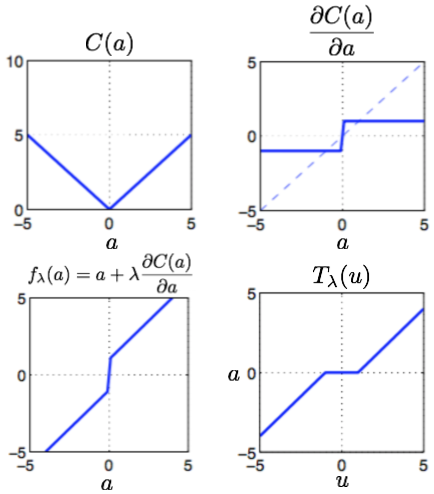
\includegraphics[width=0.5\textwidth]{lca_cost_graphs.png}
\caption{\textbf{Deriving the LCA thresholding function} Starting from a pictorial view of the $l_{1}$ cost function, one can derive the self inhibition term from equation \eqref{ufunca} and invert it to see the thresholding function described in equation \eqref{thresholdfunc}. Notice that the value of $\lambda$ dictates the range of allowable sub-threshold membrane potentials, $u_{k}$, before the neuron becomes active.}
\end{figure}

In addition to finding a sparse code, we are also interested in learning a set of dictionary elements, $\Phi$. This can be done by performing gradient descent on equation \eqref{energyfunc} using the coefficient values obtained with LCA. This yields

\begin{equation}
  \Delta \phi_{k} = \eta (S - \hat{S}) a_{k},
\label{phiupdate}
\end{equation}

\noindent where $\eta$ is the learning rate and $\hat{S}$ is the image reconstruction. To recap, for a given image sample we first find our image code, $a$, for a fixed dictionary, $\Phi$, and then using that code to update the dictionary with equation \eqref{phiupdate}.


\subsection{Convolutional LCA}
LCA can be easily extended to a convolutional varient. Interestingly, overcompleteness is not dependent on the size of the patch.

Convolutional LCA with overlap produce more stable code %[https://docs.google.com/presentation/d/1KwbbopmrRVMpExG8Gen5XjE8VFnqUDT11EztMBgS97A/edit#slide=id.g985873ba_04295 slide 16]


\subsection{Postdictions from the LCA}
linear RFS, extra classical RFS


\section{Properties of LCA trained on natural images}


\subsection{Features learned}
dictionary plot, summary plots, angle histograms, vary overcompleteness


\subsection{LCA neuron responses to natural images during inference}
inference traces / losses


\section{Alternative image coding models}


\subsection{The linear / non-linear neuron model}
Simoncelli, etc. Adding components.


\subsection{Autoencoders}
Autoencoders as a NN implementation of L/NL neurons.


\subsection{Predictive coding}
LCA is very similar to the Rao & Ballard predictive coding model.
Rao & Ballard PC.


\subsection{ICA}
LCA is an extension of ICA.
Sparse coding and ICA are related algorithms that employ similar linear generative models, but differ critically in their encoding processes. The image code produced by ICA is computed linearly, whereas sparse coding computes the code with a nonlinear inference process. Here we show that this nonlinear encoding process confers a considerable advantage in coding efficiency and orientation selectivity.

ICA assumes the generative model:

\begin{equation}
\mathbf{s} = \mathbf{\Phi a}
\end{equation}

where $\mathbf{s}$ is an image, $\mathbf{\Phi}$ is a matrix of filters and $\mathbf{a}$ is a vector of activations that represents the neural code \parencite{bell:1997gx}. The goal of ICA is to learn a set of statistically independent filters such that the input data can be reconstructed with minimal error. In ICA, the filter matrix is square and full rank and thus invertible. This allows the ICA activations for a given input to be computed directly as:

\begin{equation}
\mathbf{\hat{a}} = \mathbf{\Phi}^{-1}\mathbf{s}
\end{equation}

During inference, activations are computed with a single, linear, feed-forward operation. The filter matrix is learned via a non-linear, iterative optimization process to accurately reconstruct the input while maximizing the statistical independence of the filters as measured by the joint entropy of the activations. This process results in filters that are optimized for the higher-order statistical structure in natural scenes.

The primary objective of sparse coding, as described in Olshausen and Field (1996), is to encode input data (e.g. an image of a natural scene) in a generative framework, such that the data can be reconstructed from the code. In other words, the goal is to minimize an energy function that requires both a faithful and efficient representation of the data, in that it reconstructs the data well with the fewest number of active elements. Learning the basis functions is accomplished by maximizing the average log-likelihood of the model via gradient ascent. This optimization requires sampling from the posterior (the probability of the image given all possible codes of the image), which can be very slow (if not impossible). In practice we take a single sample at the posterior maximum. This is effectively the same as using the maximum of a distribution to represent the area under the distribution. This can be a fair assumption if the distribution is highly kurtotic (peaky), which ours is expected to be. The overall learning procedure thus involves a fast inner loop in which the coefficients are computed for each data vector and a slower outer loop in which the basis functions are adapted to the statistics of the entire dataset. In the inner loop, coefficients are computed considering the prior on their expected distribution. In ICA, however, the prior plays no role in determining the coefficients, but it does still play an important role in the learning the basis functions.

The ICA learning algorithm is simpler and faster than the sparse coding algorithm because the encoding can be computed from the data in a single feedforward pass. The basis functions are then learned by computing the cost on the code directly. The independent component analysis algorithm of Bell and Sejnowski is formally equivalent to maximum likelihood in the case of no noise and a square system (dimensionality of output = dimensionality of input). It is easy to generalize this to the case when the number of outputs is less than the number of inputs, but not the other way around. When the number of outputs is greater than the effective dimensionality of the input of non zero eigenvalues of the input covariance matrix then the extra dimensions of the output will simply drop out. While this does not pose a problem for blind separation problems where the number of independent sources is less than or equal to the number of mixed signals, it will become a concern in the representation of images, where overcompleteness is a desirable feature (Simoncelli et al., 1992). The main difference between the Olshausen and Field (1996) sparse coding model and the ICA algorithm of Bell and Sejnowski (1995) is in the simplifying assumptions they make in order to deal with the intractable integration problem posed by finding the set of basis functions that maximize the likelihood of the inputs given the model defined by those basis functions. Olshausen and Field’s algorithm assumes low-noise and thus a peaky, unimodal distribution on the joint probability between the image and the sparse code given the model in order to justify evaluating it at the maximum (MLE), whereas Bell and Sejnowski limit the dimensionality of the code to equal the dimensionality of the input and also assume no noise so that the integral becomes tractable.
